\section{Applied $\pi$-Calculus}
%Short - examples of the applied $\pi$-calculus 
%\begin{itemize}
%  \item General about Applied Pi Calculus, and how it differs from pi calculus (terms; in particular for security protocols)
%  \item Examples of applied pi calculus (handshake protocol?)
%  \item ProVerif - automatic symbolic protocol verifier
%\end{itemize}

% missing link from the unformal way of Alice and Bob notation (but more convenient), to the more formal applied pi-calculus
% "The previous chapter describes how messages exchanged in cryptographic protocols can be represented as terms. In this chapter, we discuss how the protocols themselves can be modelled."
The applied pi-calculus is based upon the language pi-calculus, but offers a more convenient use for modelling security protocols to be specified, by allowing for a more wide variety of complex primitives. It is used for describing and analysing security protocols, as it provides a more intuitive process syntax for detailing the actions of the participants in a protocol \autocite{AplliedPiCalsulus2010}. This is done by introducing the before mentioned rich term algebra for modelling the cryptographic operations used in security protocols, where function symbols represent cryptographic protocols. 

Tools such as ProVerif \autocite{ProVerif} uses a syntax closely related to the applied pi-calculus, and offers a way of automated reasoning about the security properties found in cryptographic protocols. The ProVerif tool is however not used for this report, but is mentioned as it is often used when analysing security protocols, and works as motivation for describing Applied pi-calculus, as ProVerif will most likely be used in the following thesis.\\
%- The properties of these primitives are modelled by equations \\ 
%\newpage
%"The applied pi calculus (...) is a language for describing concurrent processes and their interactions". \\
\subsection{Syntax}
The applied pi-calculus has two types of processes, the \textit{plain} and \textit{extended} process. First we introduce the grammar for the \textit{plain} process:  %(by \citeauthor{AplliedPiCalsulus2010}): 
\begin{center}
	\begin{tabular} { l l }
 		$P,\ Q,\ R$ ::= & plain processes \\ 
 		\quad $|$ 0 & null process \\  
 		\quad $|$ $P\ |\ Q$ & parallel composition \\
 		\quad $|$ !$P$ & replication \\
		\quad $|$ $\nu n.P$ & name restriction \\
		\quad $|$ if \textit{M = N} then \textit{P} else \textit{Q} & conditional \\
		\quad $|$ $u(x).P$ & message input \\
		\quad $|$ $\overline{u}\langle M\rangle .P $ & message output 
	\end{tabular}
\end{center}
The 0 process is the process that does nothing; $P\ |\ Q$ is the parallel composition of the processes \textit{P} and \textit{Q} executed in parallel; !$P$ is the replication of \textit{P} that allows for an infinite composition of $P\ |\ P\ |\ ...,$ which is often used for illustrating an unbound number of sessions; Name restriction $\nu n.P$ acts as a binder which generates a restricted name \textit{n} inside \textit{P}. This is often used for capturing fresh random numbers such as nonces and keys, or private channels, which we will see later when we apply it to the Needham-Schroeder public key Protocol; The conditional if \textit{M = N} then \textit{P} else \textit{Q} is like the one we know from normal conditioning in data types, where it behaves as \textit{P} whenever \textit{M = N} (representing equality), and as \textit{Q} otherwise; Last we have the message input and output, where $u(x).P$ expects an input on channel \textit{u} and binds it to variable \textit{x} in \textit{P}, and $\overline{u}\langle M\rangle .P $ outputs term \textit{M} on channel \textit{u} and then behaves as \textit{P}. It should be noted that message input and output will also we written as in\textit{(u, x).P} and out\textit{(u, M).P}, and parallel composition as $P\ ||\ Q$, as done by \citeauthor{DBLP:journals/ftpl/CortierK14} \\
\iffalse
Plain processes are generated by the grammar given
in Figure 5.1, where t, t1, t2, . . . range over terms, n over names, x over
variables and u is a meta-variable that stands for either a name or a
variable of channel sort. 
\fi

% Extension
\noindent The \textit{extended} process uses \textit{active substitutions} to capture the knowledge exposed to the
adversarial environment: 
\begin{center}
	\begin{tabular} { l l }
 		\textit{A, B, C} ::= & extended processes \\ 
 		\quad $|$ \textit{P} & plain process \\  
 		\quad $|$ $A\ |\ B$ & parallel composition \\
		\quad $|$ $\nu n.A$ & name restriction \\
		\quad $|$ $\nu x.P$ & variable restriction \\
		\quad $|$ $\{ \sfrac{M}{x} \}$ & active substitution
	\end{tabular}
\end{center}
With \textit{active substitution} we allow for \textit{M} to be available in the environment through the 'handle' \textit{x}. In other words, \textit{M} can now be replaced by \textit{x} in every process it is related to, and is only controlled by the variable restriction, i.e. $\nu x.(\{\sfrac{M}{x}\}\ |\ P)$ is exactly the same as writing $x$ = $M$ in $P.$\\ 
%Terms

\noindent With terms we use function symbols to capture primitives such as encryption or decryption used by cryptographic protocols. It should be noted that functions with arity 0 are what we define as constants.
For terms we apply function symbols to names, variable and other terms as such: 
\begin{center}
	\begin{tabular} { l l }
 		L, M, N, T, U, V ::= & terms \\ 
 		\quad $|$ a, b, c,...,k,...,m, n,..,s & names \\  
 		\quad $|$ x, y, z & variables \\
 		\quad $|$ g(M$_{1}$,..,M$_{l}$) & function application
		%\caption{Fig. 1.1}
		%\label{tbl:excel-table}
	\end{tabular}
\end{center}
These three grammars work as the foundation for applied pi-calculus, which in itself is a fairly simple language but the capabilities of describing security protocols in more detail than presented earlier. 

\subsection{Re-visiting the Needham-Schroeder Protocol}
Having established an understanding of the applied pi-calculus and its grammar, we now use it model the previously mentioned Needham-Schroeder public key protocol.\\

\noindent To make a more detailed illustration, the processes has been parametrised to represent the initiator (Alice) and responder (Bob). First we look at the process of Alice (\textit{P$_A$}):
\begin{center}
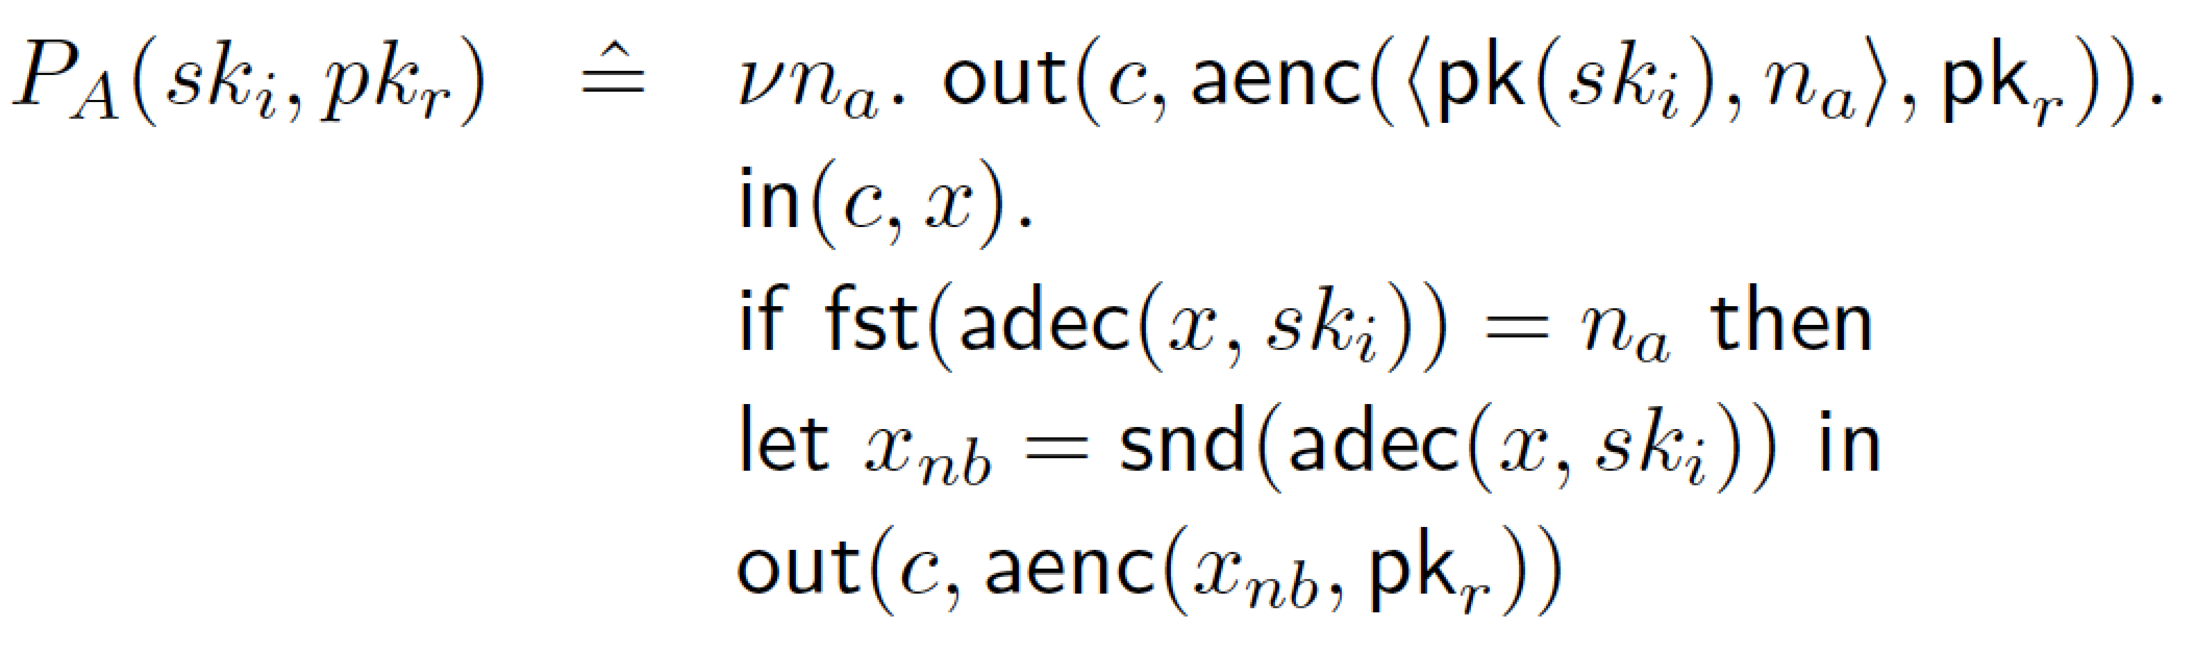
\includegraphics[width=0.65\textwidth, angle=0]{Graphics/P_A.pdf}
\end{center}
The first thing Alice does is to generate a fresh random nonce and binds it to \textit{n$_a$}, the process then continues to output the first message of an asymmetric encryption on channel \textit{c}. Next she waits for a input message on the same channel, and binds the message to variable \textit{x}. She then checks wether the message matches her previously sent nonce \textit{n$_a$} shown as the conditional. For readability the \textit{x} is then bound to a local variable \textit{n$_{xb}$}, representing the nonce received by the sender (Bob). Last she sends out a message again with an encryption of Bob's nonce and the public key, on channel \textit{c}.

The dual of the process can now be modelled from the responder's (Bob) point of view:
\begin{center}
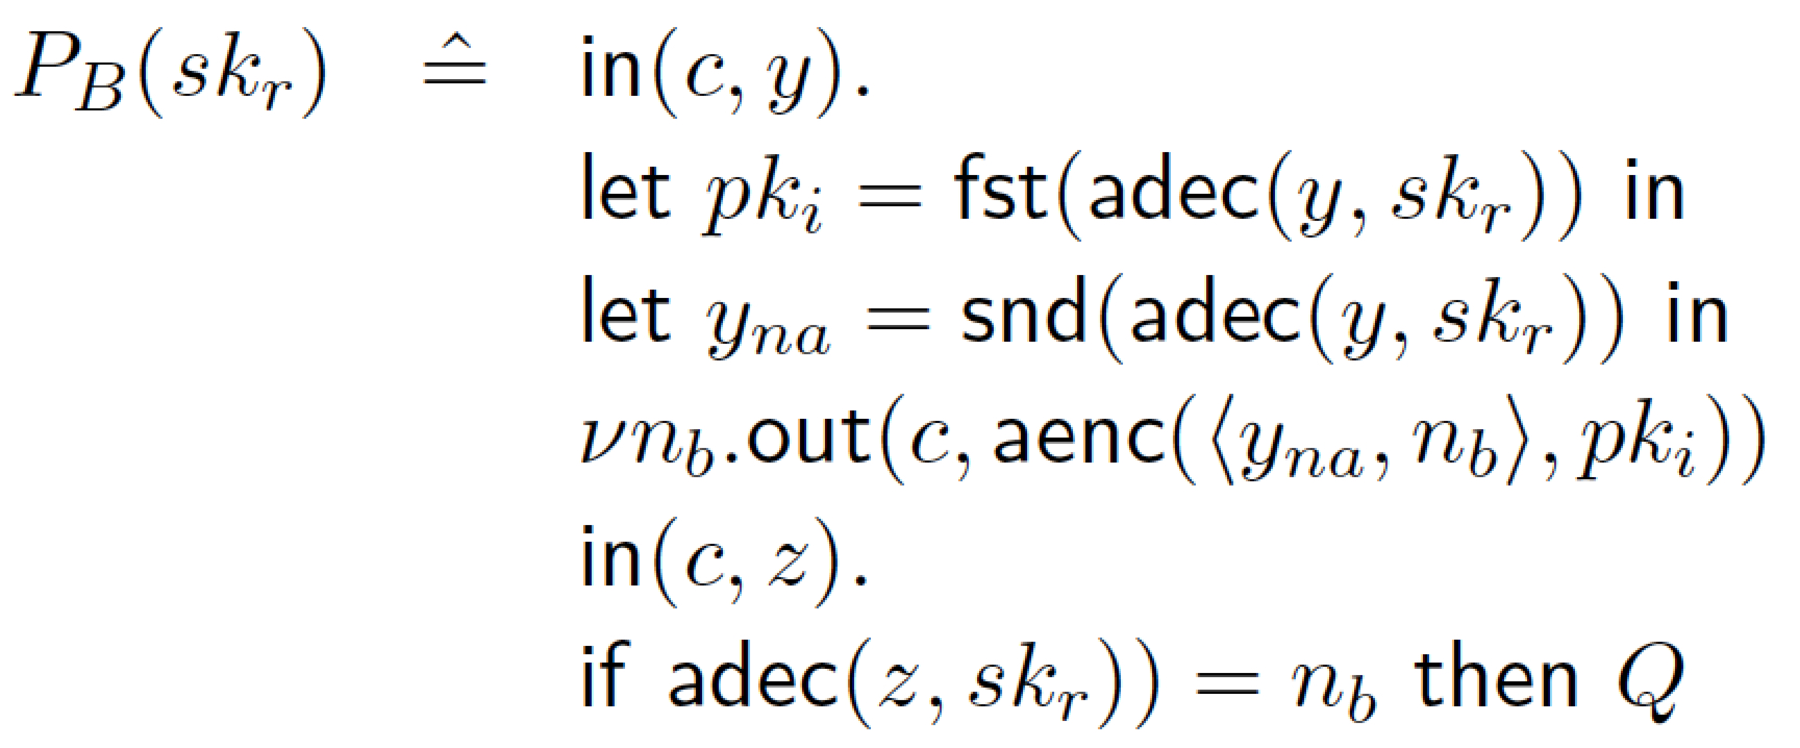
\includegraphics[width=0.55\textwidth, angle=0]{Graphics/P_B.pdf}
\end{center}

\noindent Combining the two processes we are able to model the Needham-Schroeder public key protocol, done so by \citeauthor{DBLP:journals/ftpl/CortierK14}, as a whole: 
\begin{center}
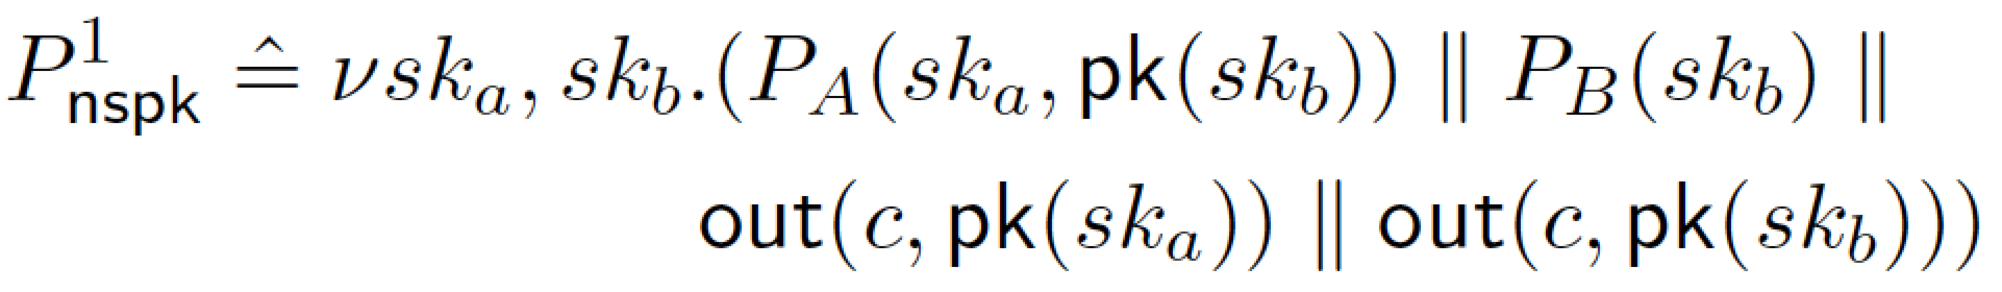
\includegraphics[width=0.6\textwidth, angle=0]{Graphics/P1_nspk.pdf}
\end{center}
This however represent the naive model of the protocol, so to add the Lowe fix, as mentioned earlier i then report, we need to modify the protocol slightly:
\begin{center}
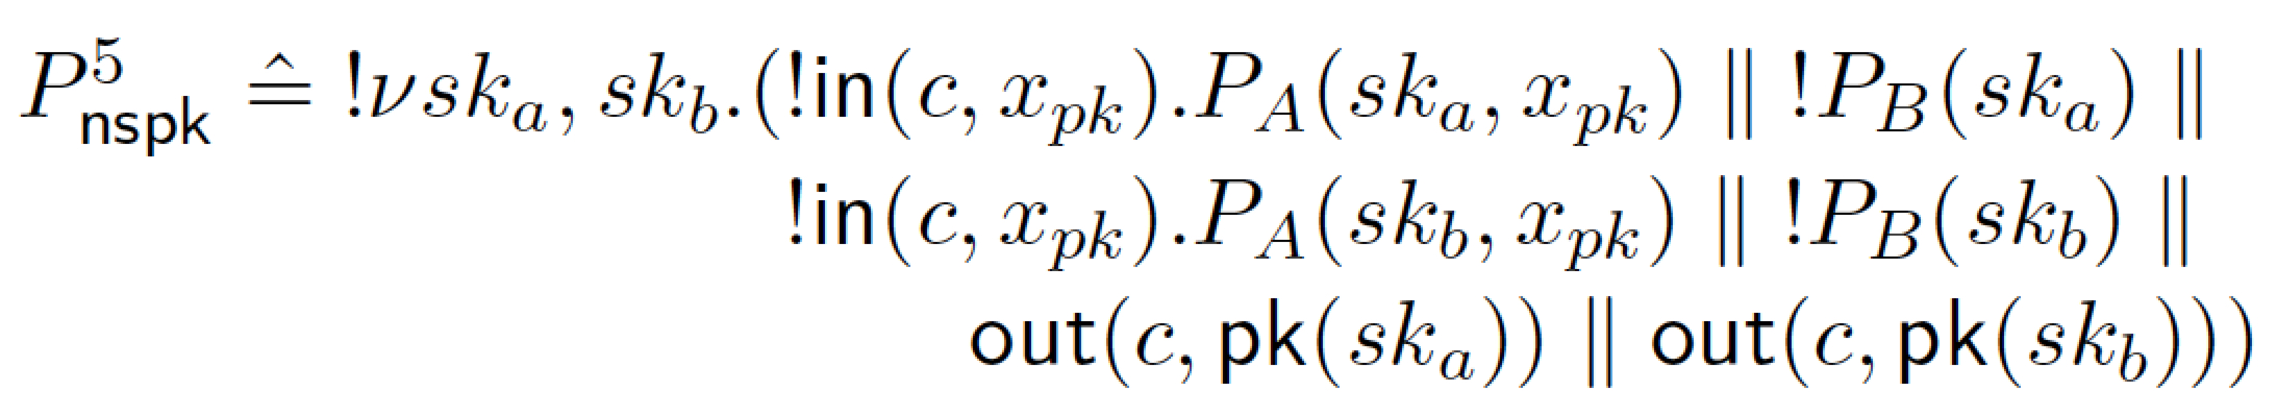
\includegraphics[width=0.6\textwidth, angle=0]{Graphics/P5_nspk.pdf}
\end{center}
As can be seen, the input of the public key by Bob, shown as pk($sk_b$), is now replaced by $x_{pk}$ representing the unknown value of the variable, illustrating how Alice does now know who she is starting a session with. This also highlight the risk of an \textit{reflection attack}, where the intruder tricks the participant to execute a protocol with him/her self. Replication has also been added to the session, as no upper bound has been put for the number of parallel session that may be initiated. Last but not least, we showcase that both session may be started by the same participant. All of this allow for an adversary to create an arbitrary number of instances of $P_A$ and $P_B$ with either the same or different private keys \autocite{DBLP:journals/ftpl/CortierK14}. \\ \\
For the next section, we will look at another way of illustrating protocols that also have its roots from the process calculus.  


% Extra
% Handshake protocol
\iffalse
First of, we look at the simple Handshake protocol used for setting the parameters for communication between two devices, such as the old dial-up modem or when connecting to a USB.  \\
Handshake protocol with applied pi-calculus as illustred by \citeauthor{AplliedPiCalsulus2010}:
\begin{center}
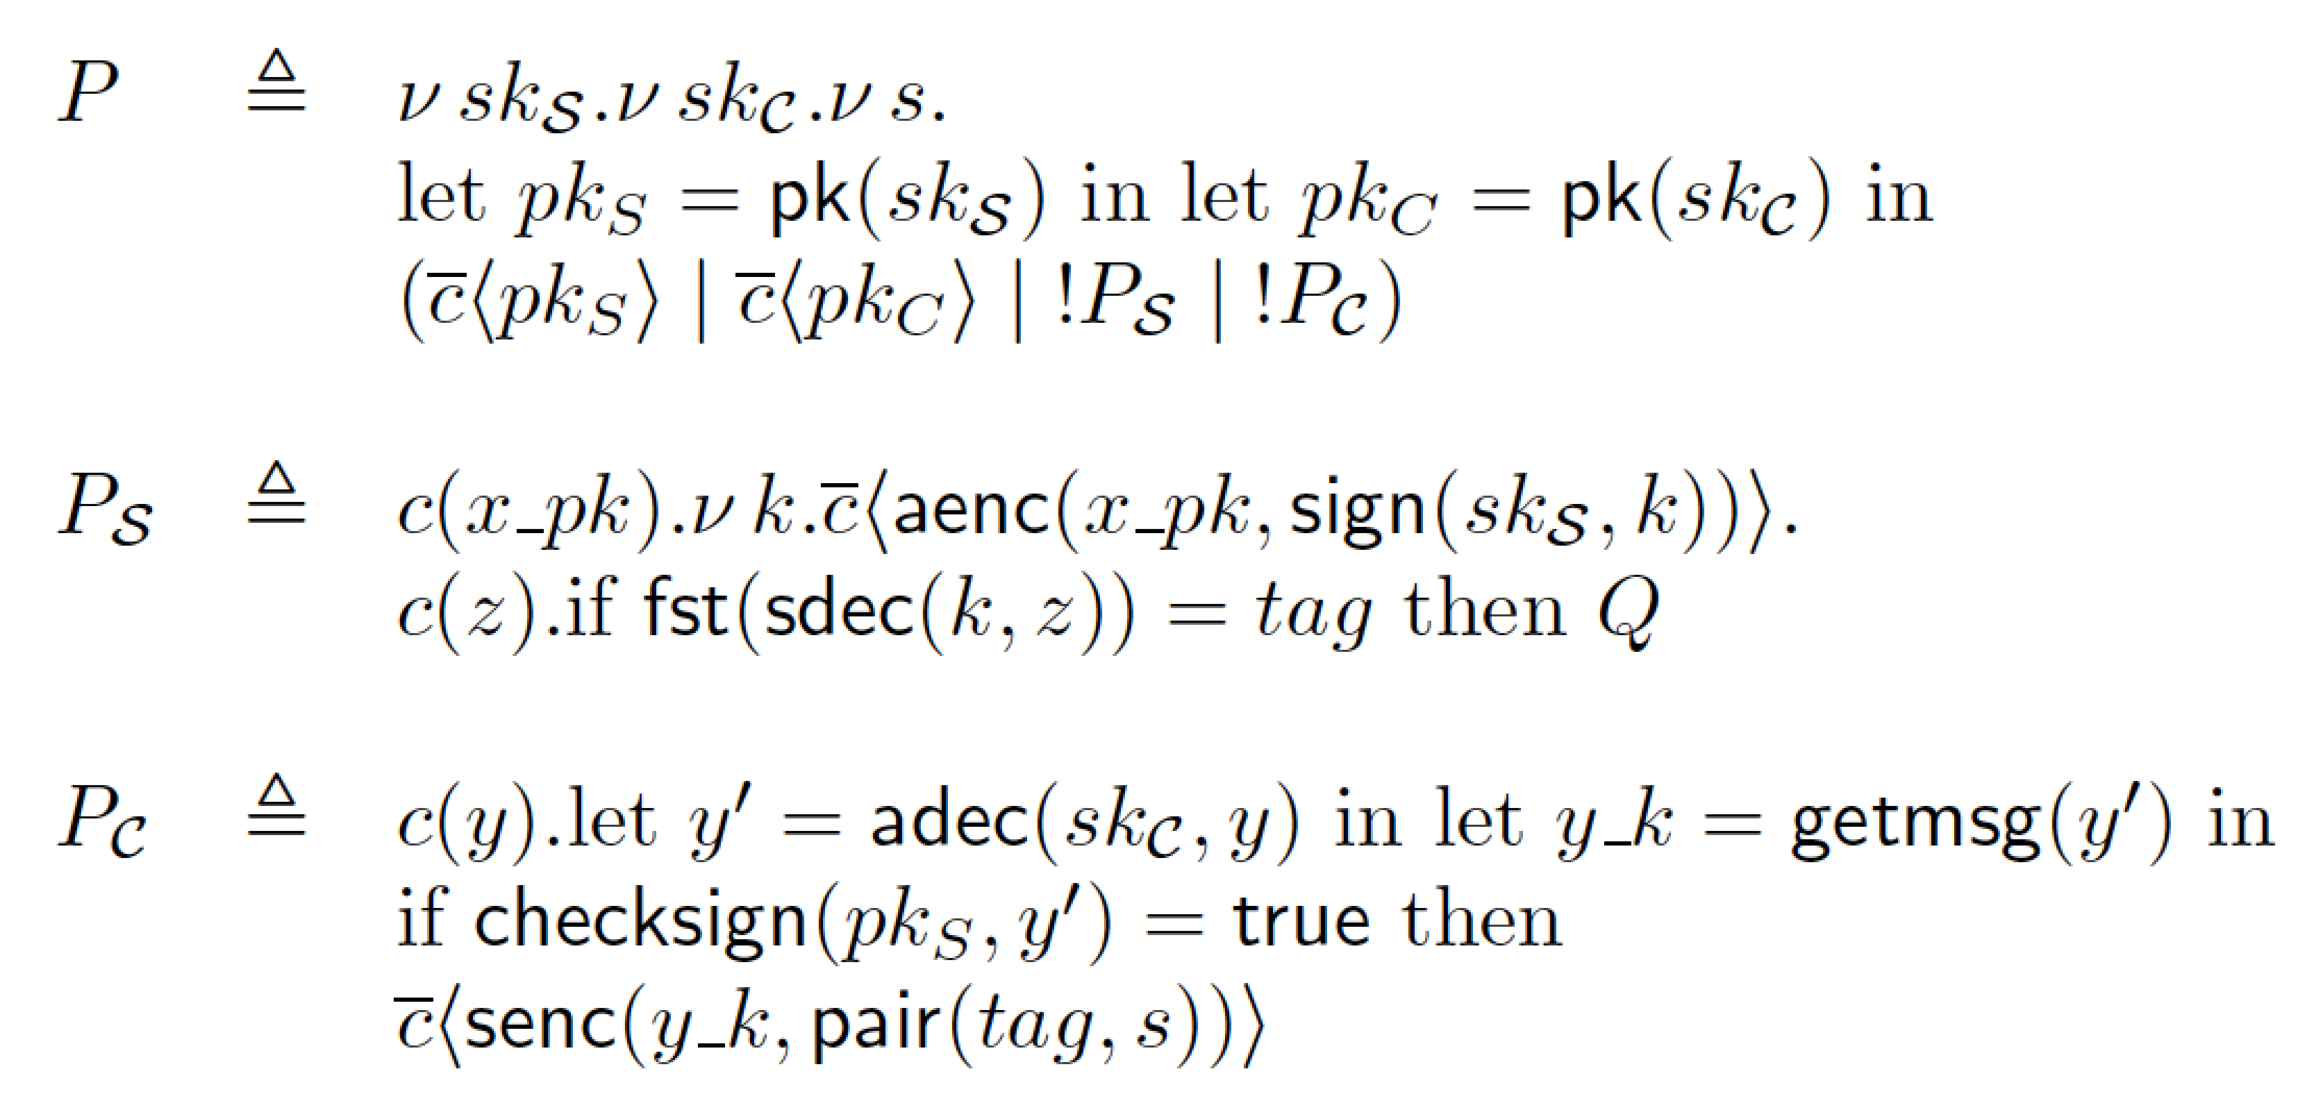
\includegraphics[width=0.75\textwidth, angle=0]{Graphics/Handshake.pdf}
\end{center}
\fi
